% Options for packages loaded elsewhere
% Options for packages loaded elsewhere
\PassOptionsToPackage{unicode}{hyperref}
\PassOptionsToPackage{hyphens}{url}
%
\documentclass[
  ignorenonframetext,
]{beamer}
\newif\ifbibliography
\usepackage{pgfpages}
\setbeamertemplate{caption}[numbered]
\setbeamertemplate{caption label separator}{: }
\setbeamercolor{caption name}{fg=normal text.fg}
\beamertemplatenavigationsymbolsempty
% remove section numbering
\setbeamertemplate{part page}{
  \centering
  \begin{beamercolorbox}[sep=16pt,center]{part title}
    \usebeamerfont{part title}\insertpart\par
  \end{beamercolorbox}
}
\setbeamertemplate{section page}{
  \centering
  \begin{beamercolorbox}[sep=12pt,center]{section title}
    \usebeamerfont{section title}\insertsection\par
  \end{beamercolorbox}
}
\setbeamertemplate{subsection page}{
  \centering
  \begin{beamercolorbox}[sep=8pt,center]{subsection title}
    \usebeamerfont{subsection title}\insertsubsection\par
  \end{beamercolorbox}
}
% Prevent slide breaks in the middle of a paragraph
\widowpenalties 1 10000
\raggedbottom
\AtBeginPart{
  \frame{\partpage}
}
\AtBeginSection{
  \ifbibliography
  \else
    \frame{\sectionpage}
  \fi
}
\AtBeginSubsection{
  \frame{\subsectionpage}
}
\usepackage{iftex}
\ifPDFTeX
  \usepackage[T1]{fontenc}
  \usepackage[utf8]{inputenc}
  \usepackage{textcomp} % provide euro and other symbols
\else % if luatex or xetex
  \usepackage{unicode-math} % this also loads fontspec
  \defaultfontfeatures{Scale=MatchLowercase}
  \defaultfontfeatures[\rmfamily]{Ligatures=TeX,Scale=1}
\fi
\usepackage{lmodern}

\ifPDFTeX\else
  % xetex/luatex font selection
\fi
% Use upquote if available, for straight quotes in verbatim environments
\IfFileExists{upquote.sty}{\usepackage{upquote}}{}
\IfFileExists{microtype.sty}{% use microtype if available
  \usepackage[]{microtype}
  \UseMicrotypeSet[protrusion]{basicmath} % disable protrusion for tt fonts
}{}
\makeatletter
\@ifundefined{KOMAClassName}{% if non-KOMA class
  \IfFileExists{parskip.sty}{%
    \usepackage{parskip}
  }{% else
    \setlength{\parindent}{0pt}
    \setlength{\parskip}{6pt plus 2pt minus 1pt}}
}{% if KOMA class
  \KOMAoptions{parskip=half}}
\makeatother


\usepackage{longtable,booktabs,array}
\usepackage{calc} % for calculating minipage widths
\usepackage{caption}
% Make caption package work with longtable
\makeatletter
\def\fnum@table{\tablename~\thetable}
\makeatother
\usepackage{graphicx}
\makeatletter
\newsavebox\pandoc@box
\newcommand*\pandocbounded[1]{% scales image to fit in text height/width
  \sbox\pandoc@box{#1}%
  \Gscale@div\@tempa{\textheight}{\dimexpr\ht\pandoc@box+\dp\pandoc@box\relax}%
  \Gscale@div\@tempb{\linewidth}{\wd\pandoc@box}%
  \ifdim\@tempb\p@<\@tempa\p@\let\@tempa\@tempb\fi% select the smaller of both
  \ifdim\@tempa\p@<\p@\scalebox{\@tempa}{\usebox\pandoc@box}%
  \else\usebox{\pandoc@box}%
  \fi%
}
% Set default figure placement to htbp
\def\fps@figure{htbp}
\makeatother





\setlength{\emergencystretch}{3em} % prevent overfull lines

\providecommand{\tightlist}{%
  \setlength{\itemsep}{0pt}\setlength{\parskip}{0pt}}



 


\makeatletter
\@ifpackageloaded{caption}{}{\usepackage{caption}}
\AtBeginDocument{%
\ifdefined\contentsname
  \renewcommand*\contentsname{Table of contents}
\else
  \newcommand\contentsname{Table of contents}
\fi
\ifdefined\listfigurename
  \renewcommand*\listfigurename{List of Figures}
\else
  \newcommand\listfigurename{List of Figures}
\fi
\ifdefined\listtablename
  \renewcommand*\listtablename{List of Tables}
\else
  \newcommand\listtablename{List of Tables}
\fi
\ifdefined\figurename
  \renewcommand*\figurename{Figure}
\else
  \newcommand\figurename{Figure}
\fi
\ifdefined\tablename
  \renewcommand*\tablename{Table}
\else
  \newcommand\tablename{Table}
\fi
}
\@ifpackageloaded{float}{}{\usepackage{float}}
\floatstyle{ruled}
\@ifundefined{c@chapter}{\newfloat{codelisting}{h}{lop}}{\newfloat{codelisting}{h}{lop}[chapter]}
\floatname{codelisting}{Listing}
\newcommand*\listoflistings{\listof{codelisting}{List of Listings}}
\makeatother
\makeatletter
\makeatother
\makeatletter
\@ifpackageloaded{caption}{}{\usepackage{caption}}
\@ifpackageloaded{subcaption}{}{\usepackage{subcaption}}
\makeatother

\usepackage{bookmark}
\IfFileExists{xurl.sty}{\usepackage{xurl}}{} % add URL line breaks if available
\urlstyle{same}
\hypersetup{
  pdftitle={Week 1: Gen AI for Sociology},
  hidelinks,
  pdfcreator={LaTeX via pandoc}}


\title{Week 1: Gen AI for Sociology}
\author{}
\date{}

\begin{document}
\frame{\titlepage}


\begin{frame}{Course Overview}
\phantomsection\label{course-overview}
\begin{itemize}
\tightlist
\item
  goals, schedule, grading
\end{itemize}
\end{frame}

\begin{frame}{Discussion}
\phantomsection\label{discussion}
\begin{itemize}[<+->]
\tightlist
\item
  introductions
\item
  how do you use AI (LLMs)?
\item
  what are your interests?
\item
  is it stopping your from learning?
\item
  do you ever stop to question yourself?
\item
  how does it feel to be a grad. student in this moment?
\end{itemize}
\end{frame}

\begin{frame}{AI ``Policy''}
\phantomsection\label{ai-policy}
\begin{itemize}
\tightlist
\item
  Here's my thoughts\ldots{}
\end{itemize}
\end{frame}

\begin{frame}{}
\phantomsection\label{section}
\begin{center}
\pandocbounded{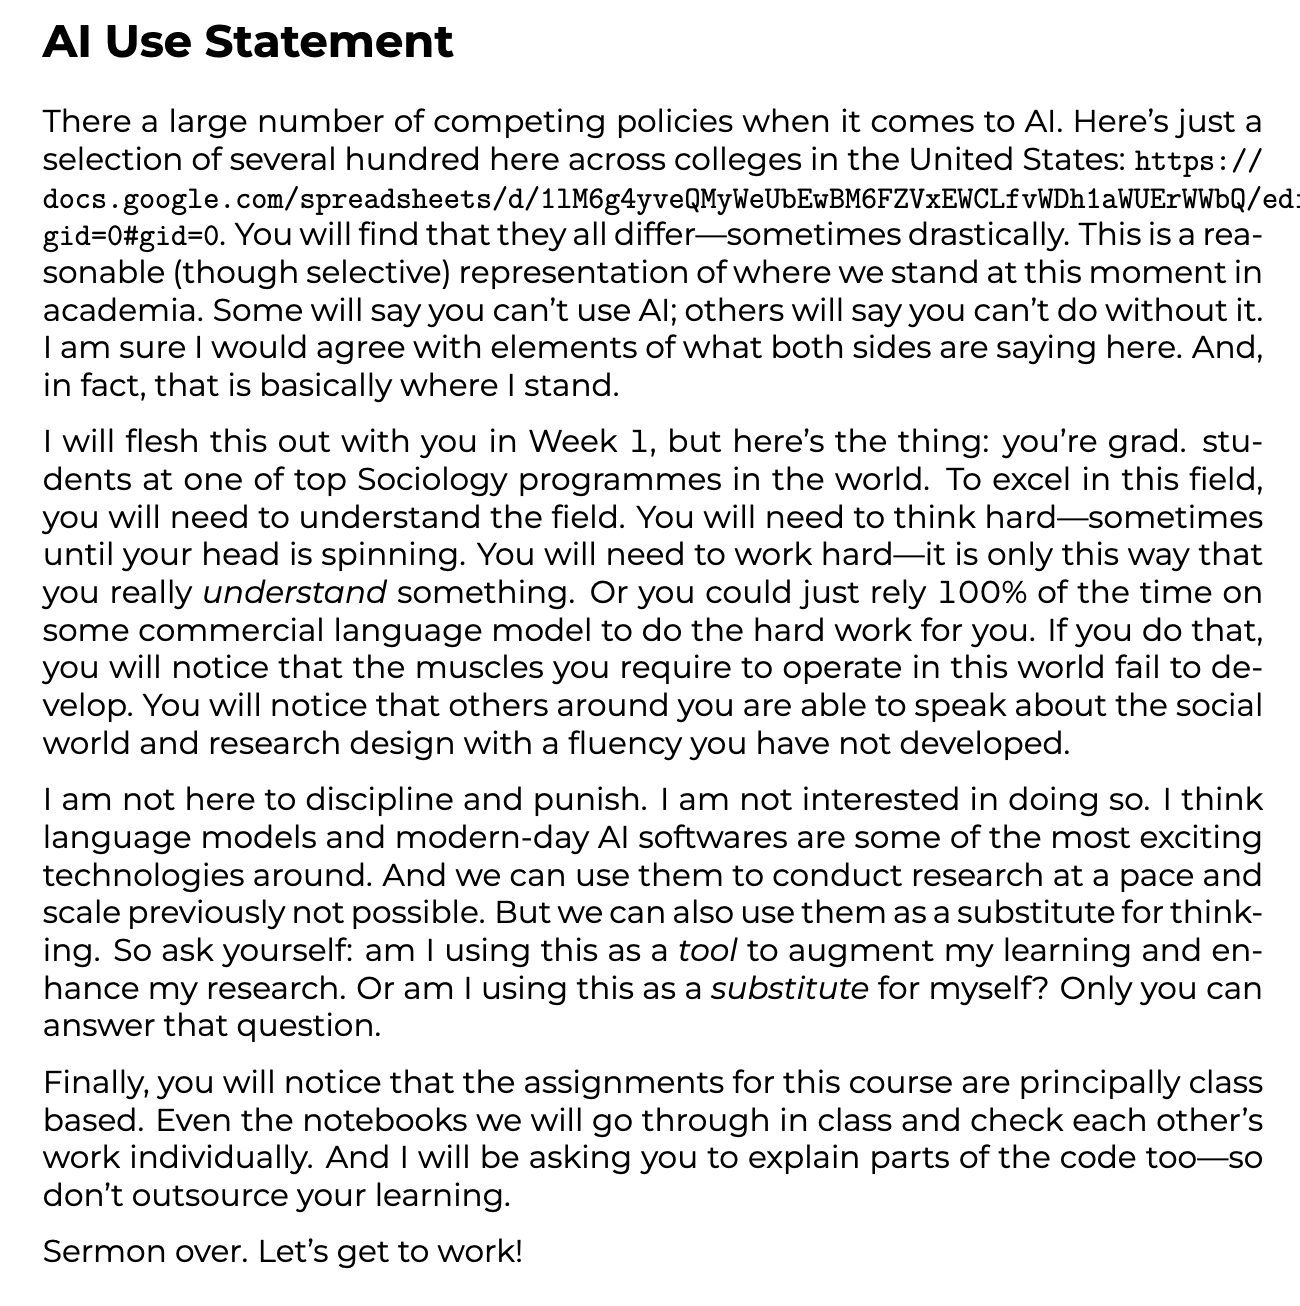
\includegraphics[keepaspectratio]{images/statement.png}}
\end{center}
\end{frame}

\begin{frame}{AI is booming}
\phantomsection\label{ai-is-booming}
\begin{center}
\pandocbounded{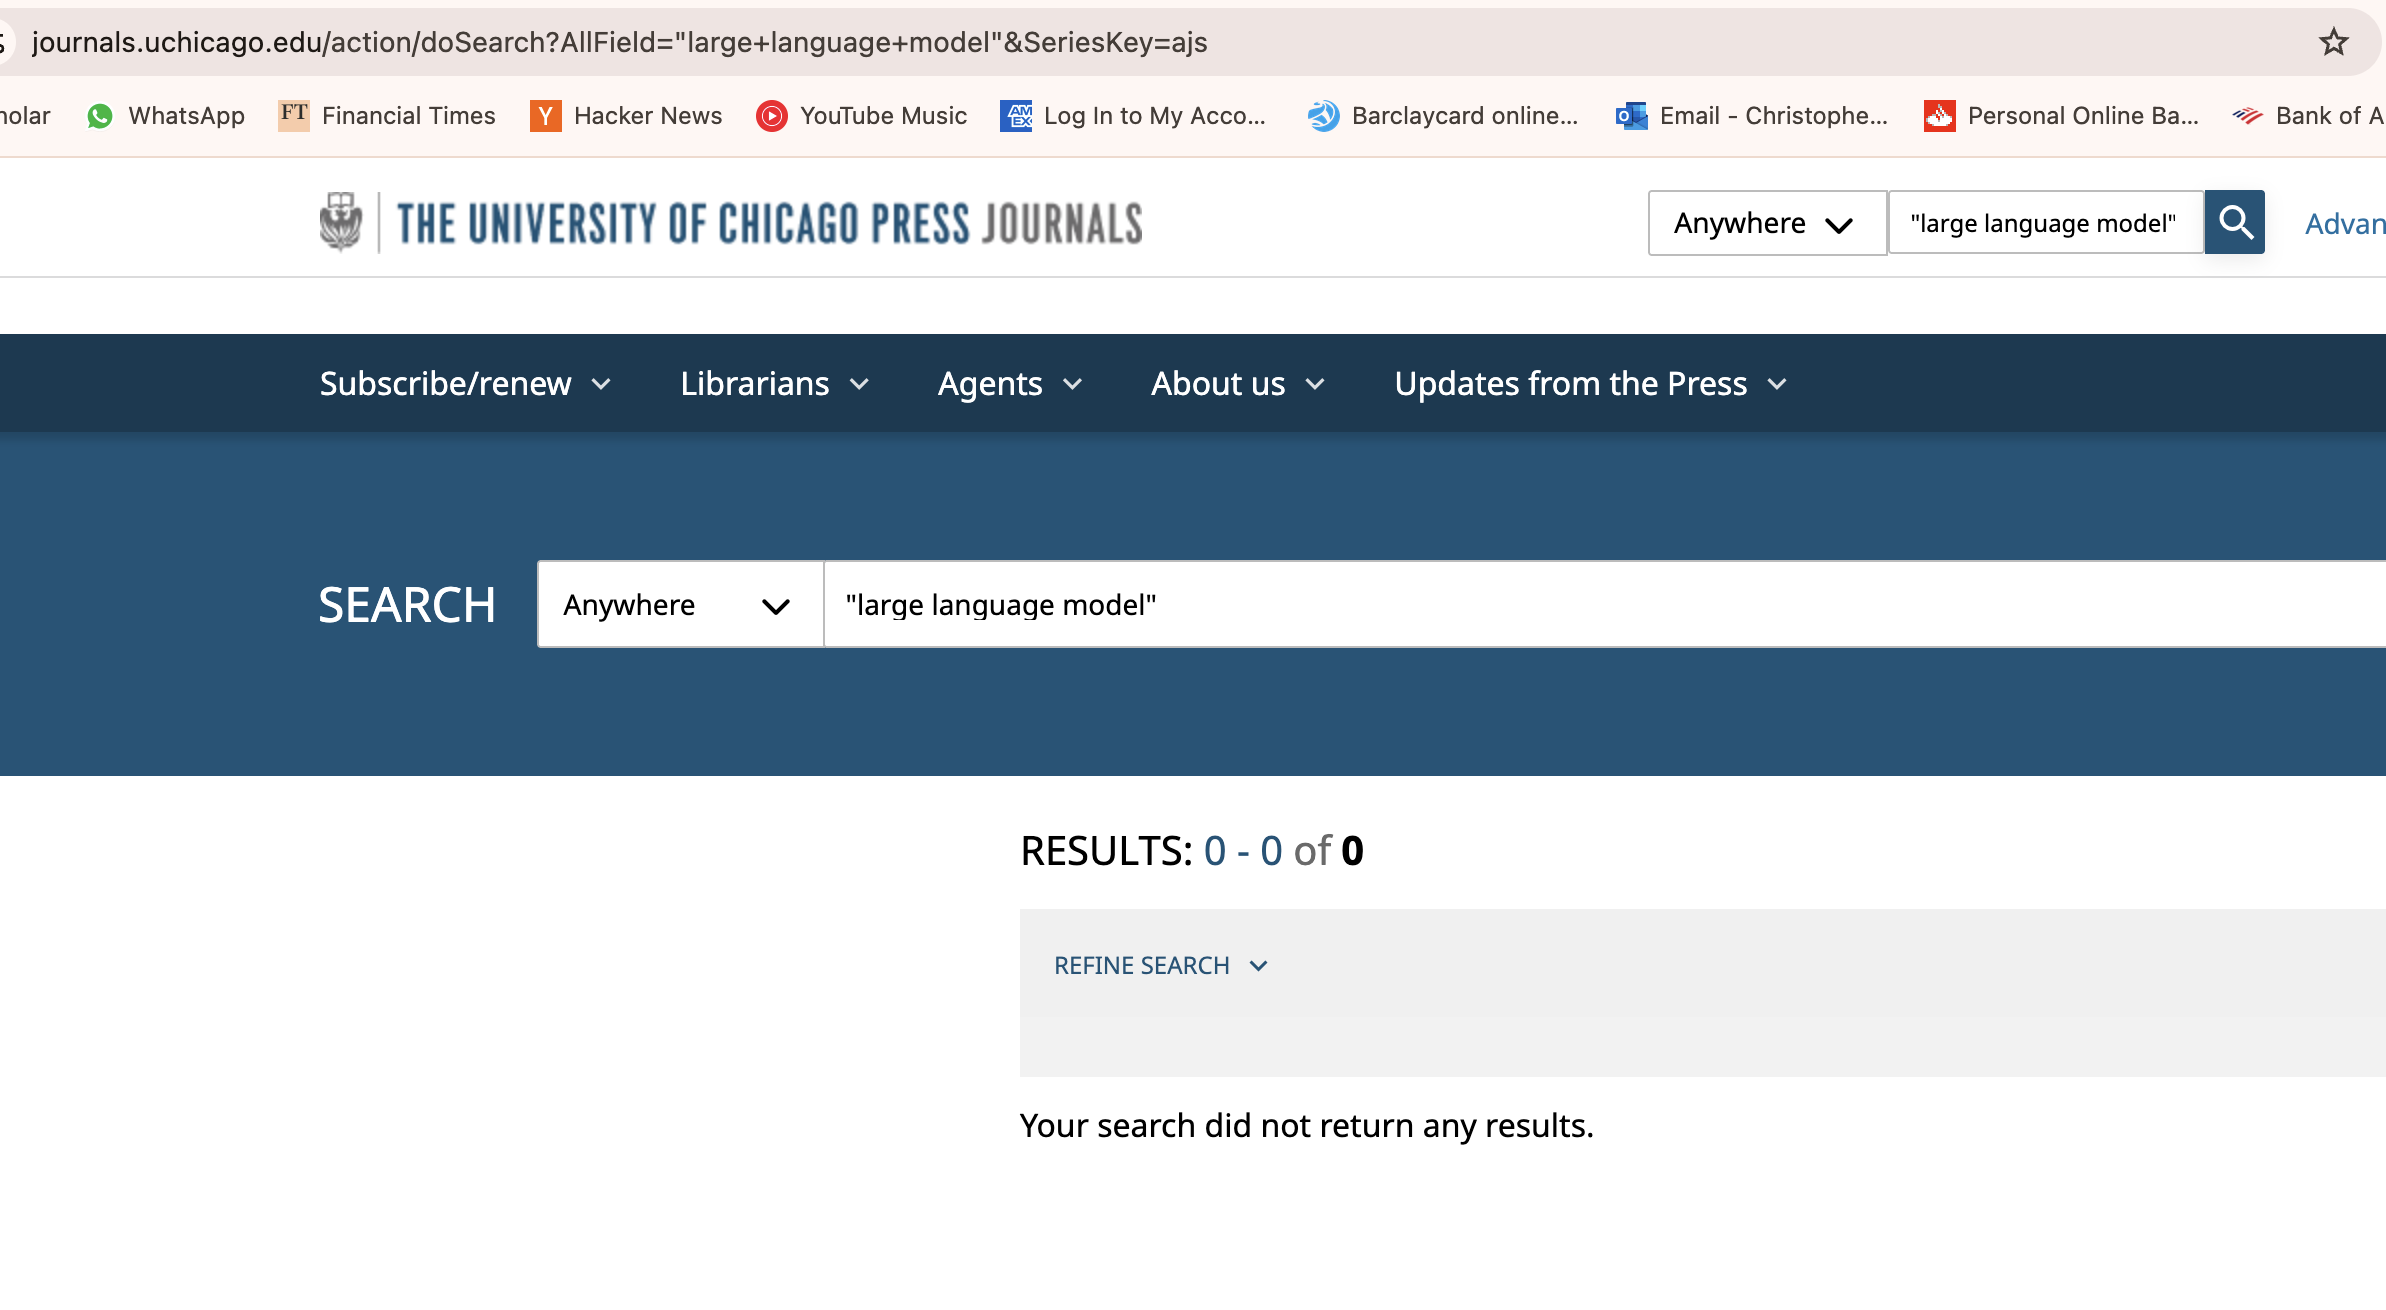
\includegraphics[keepaspectratio]{images/ajs.png}}
\end{center}
\end{frame}

\begin{frame}{AI is booming (part 2)}
\phantomsection\label{ai-is-booming-part-2}
\begin{center}
\pandocbounded{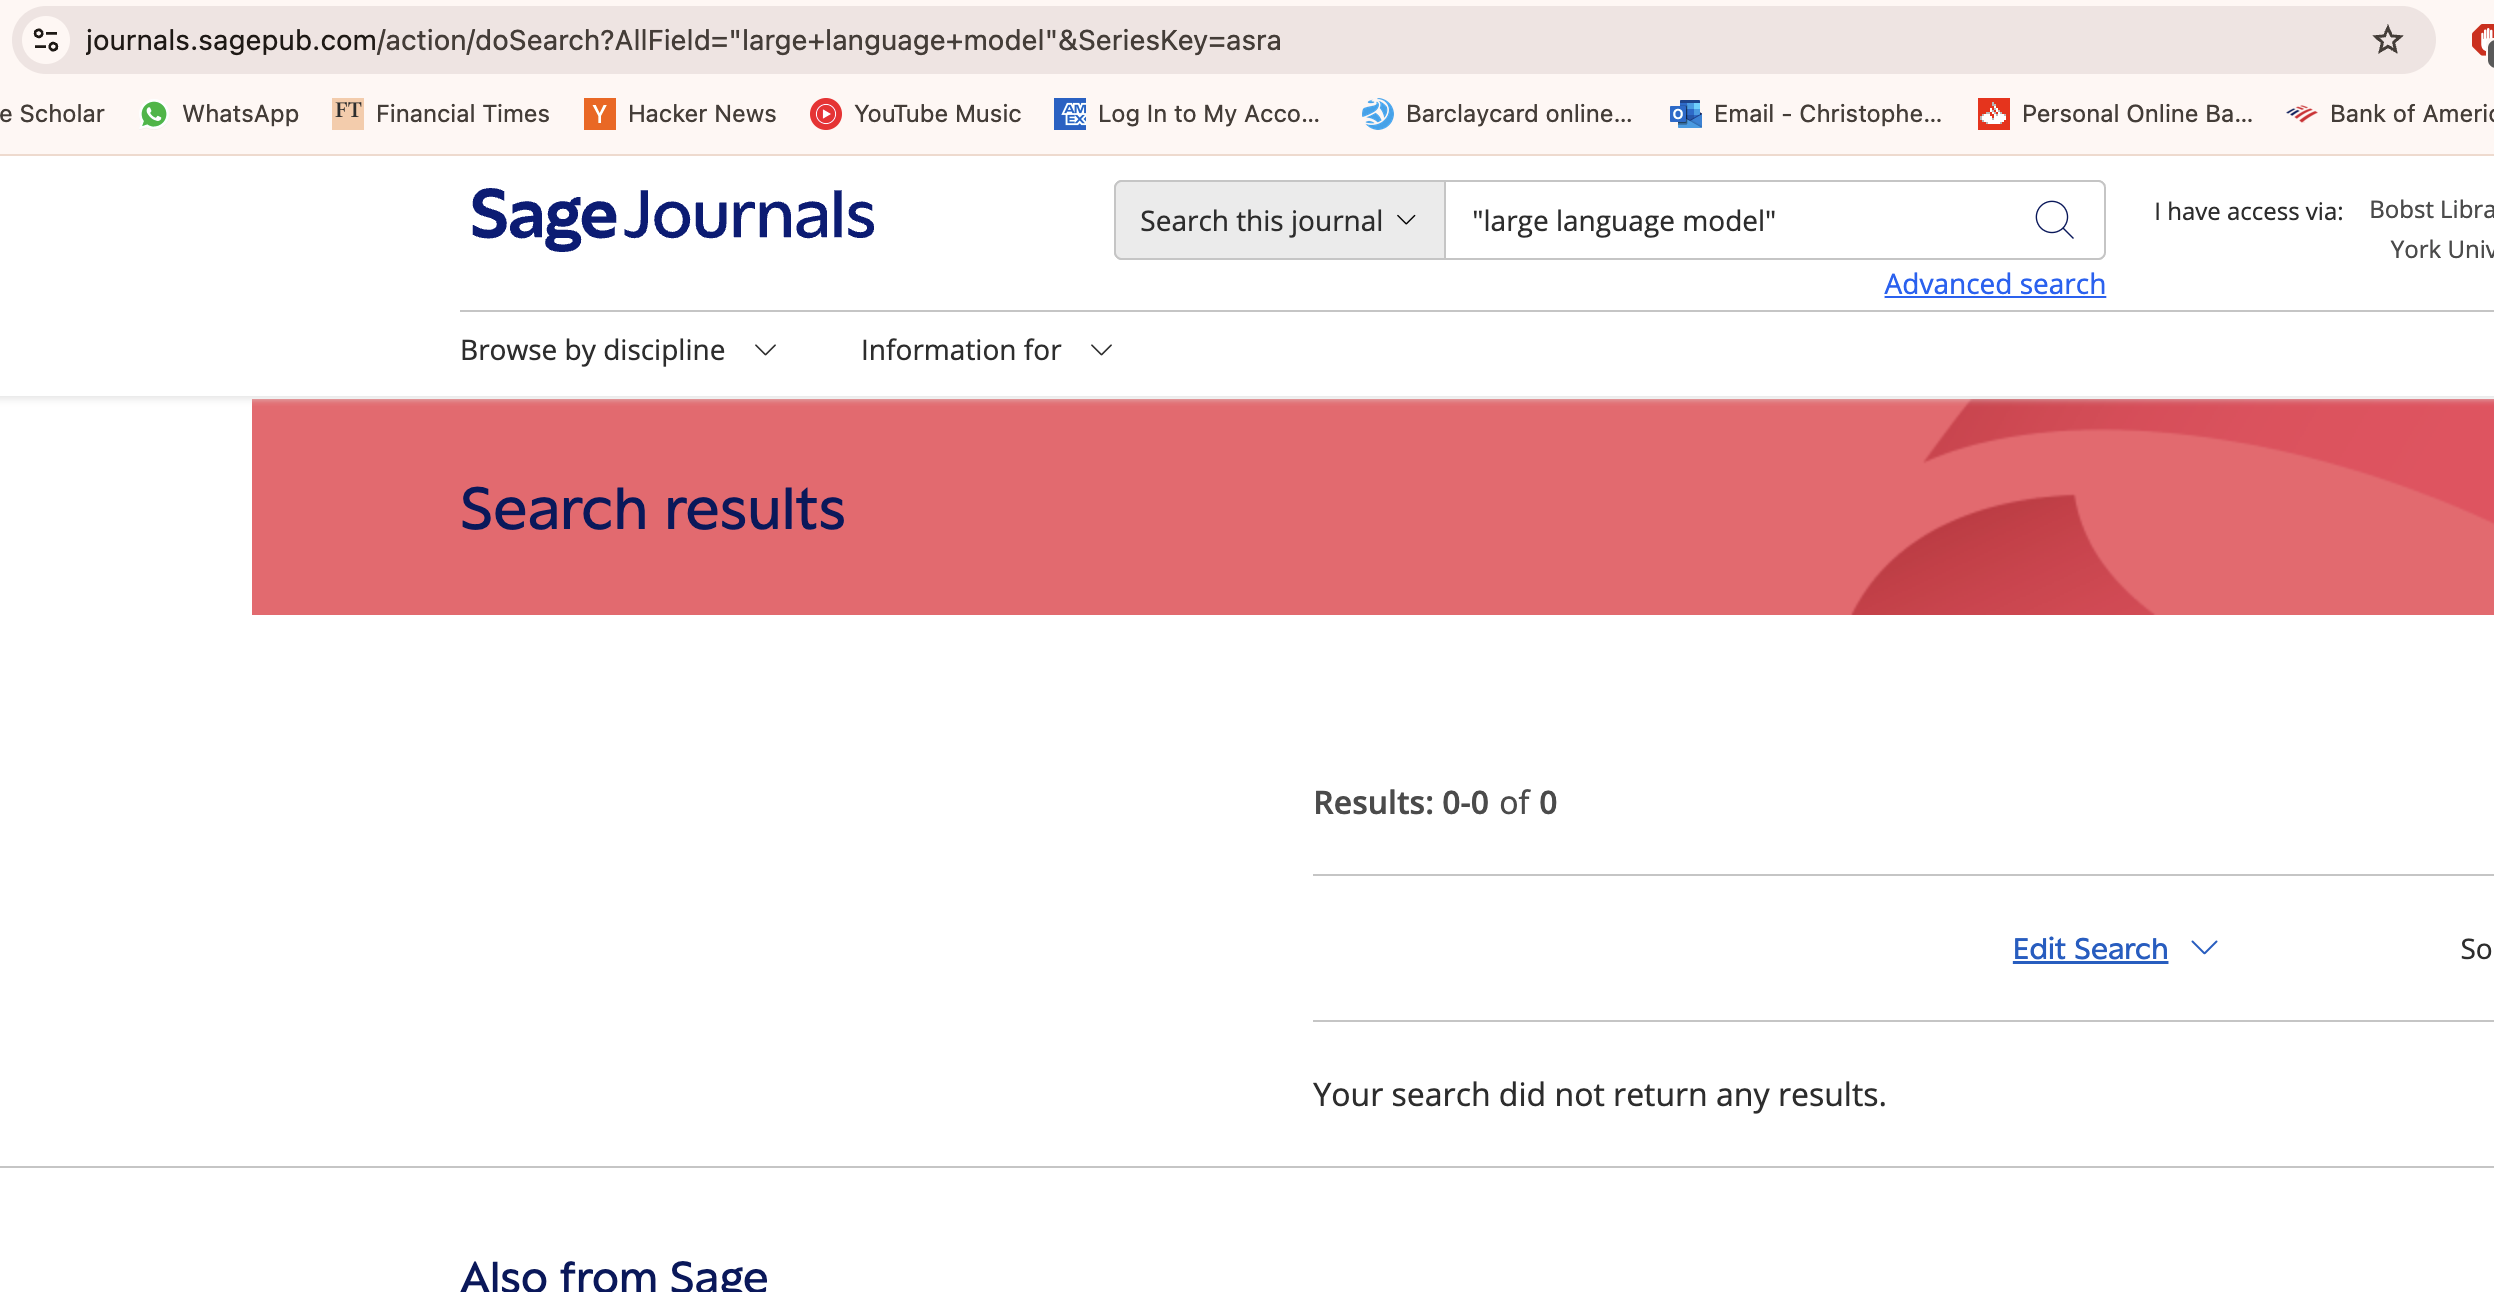
\includegraphics[keepaspectratio]{images/asr.png}}
\end{center}
\end{frame}

\begin{frame}{AI is booming (part 3)}
\phantomsection\label{ai-is-booming-part-3}
\begin{center}
\pandocbounded{
\includegraphics[keepaspectratio]{images/smr.png}}
\end{center}
\end{frame}

\begin{frame}{Where do we place all of this stuff??}
\phantomsection\label{where-do-we-place-all-of-this-stuff}
Situating the field

\begin{itemize}[<+->]
\tightlist
\item
  Text as data
\item
  Machine learning
\item
  Algorithmic bias
\item
  Simulation
\end{itemize}
\end{frame}

\begin{frame}{Text as data}
\phantomsection\label{text-as-data}
\begin{itemize}[<+->]
\tightlist
\item
  Using text as a source of data for social science research
\item
  Coding according to rules and textual features
\end{itemize}
\end{frame}

\begin{frame}{Some early examples}
\phantomsection\label{some-early-examples}
\begin{center}
\pandocbounded{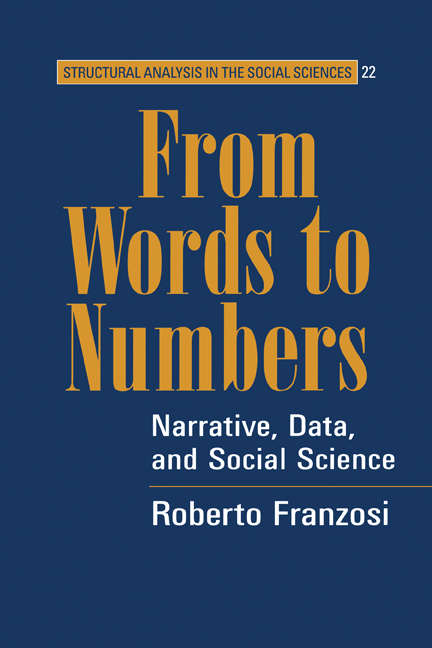
\includegraphics[keepaspectratio]{images/franzosi.png}}
\end{center}
\end{frame}

\begin{frame}{Some early examples}
\phantomsection\label{some-early-examples-1}
\begin{center}
\pandocbounded{
\includegraphics[keepaspectratio]{images/lasswell2.png}}
\end{center}
\end{frame}

\begin{frame}{Some early examples}
\phantomsection\label{some-early-examples-2}
\begin{center}
\pandocbounded{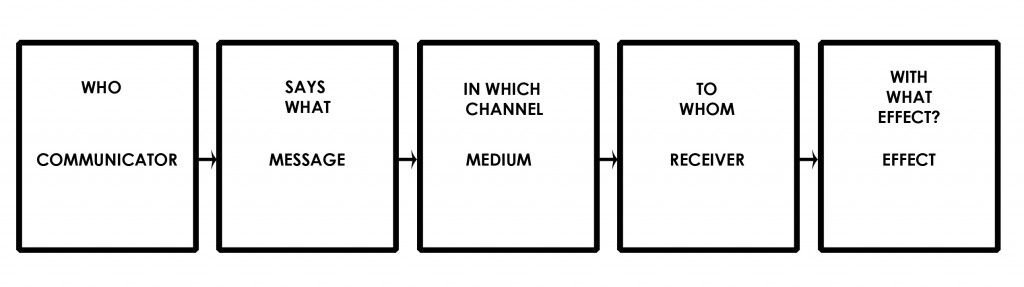
\includegraphics[keepaspectratio]{images/lasswell.png}}
\end{center}
\end{frame}

\begin{frame}{Some modern-day renewals}
\phantomsection\label{some-modern-day-renewals}
\begin{center}
\pandocbounded{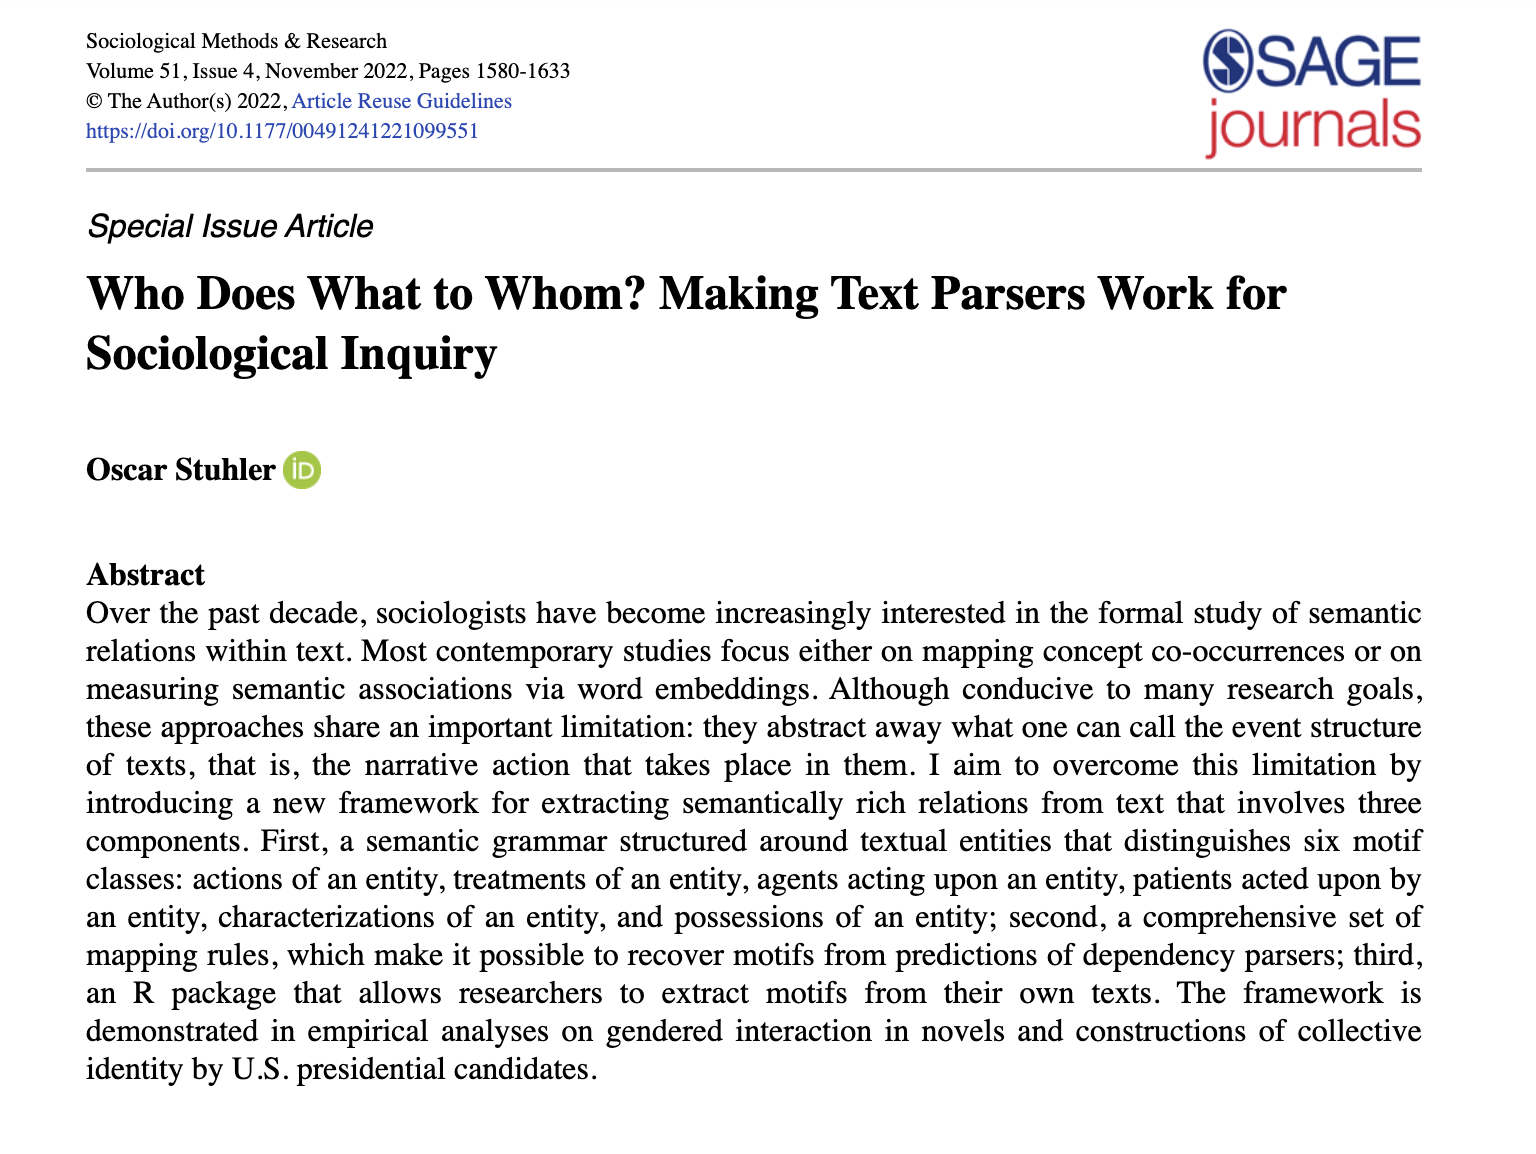
\includegraphics[keepaspectratio]{images/stuhler.png}}
\end{center}
\end{frame}

\begin{frame}{Machine learning}
\phantomsection\label{machine-learning}
\begin{center}
\pandocbounded{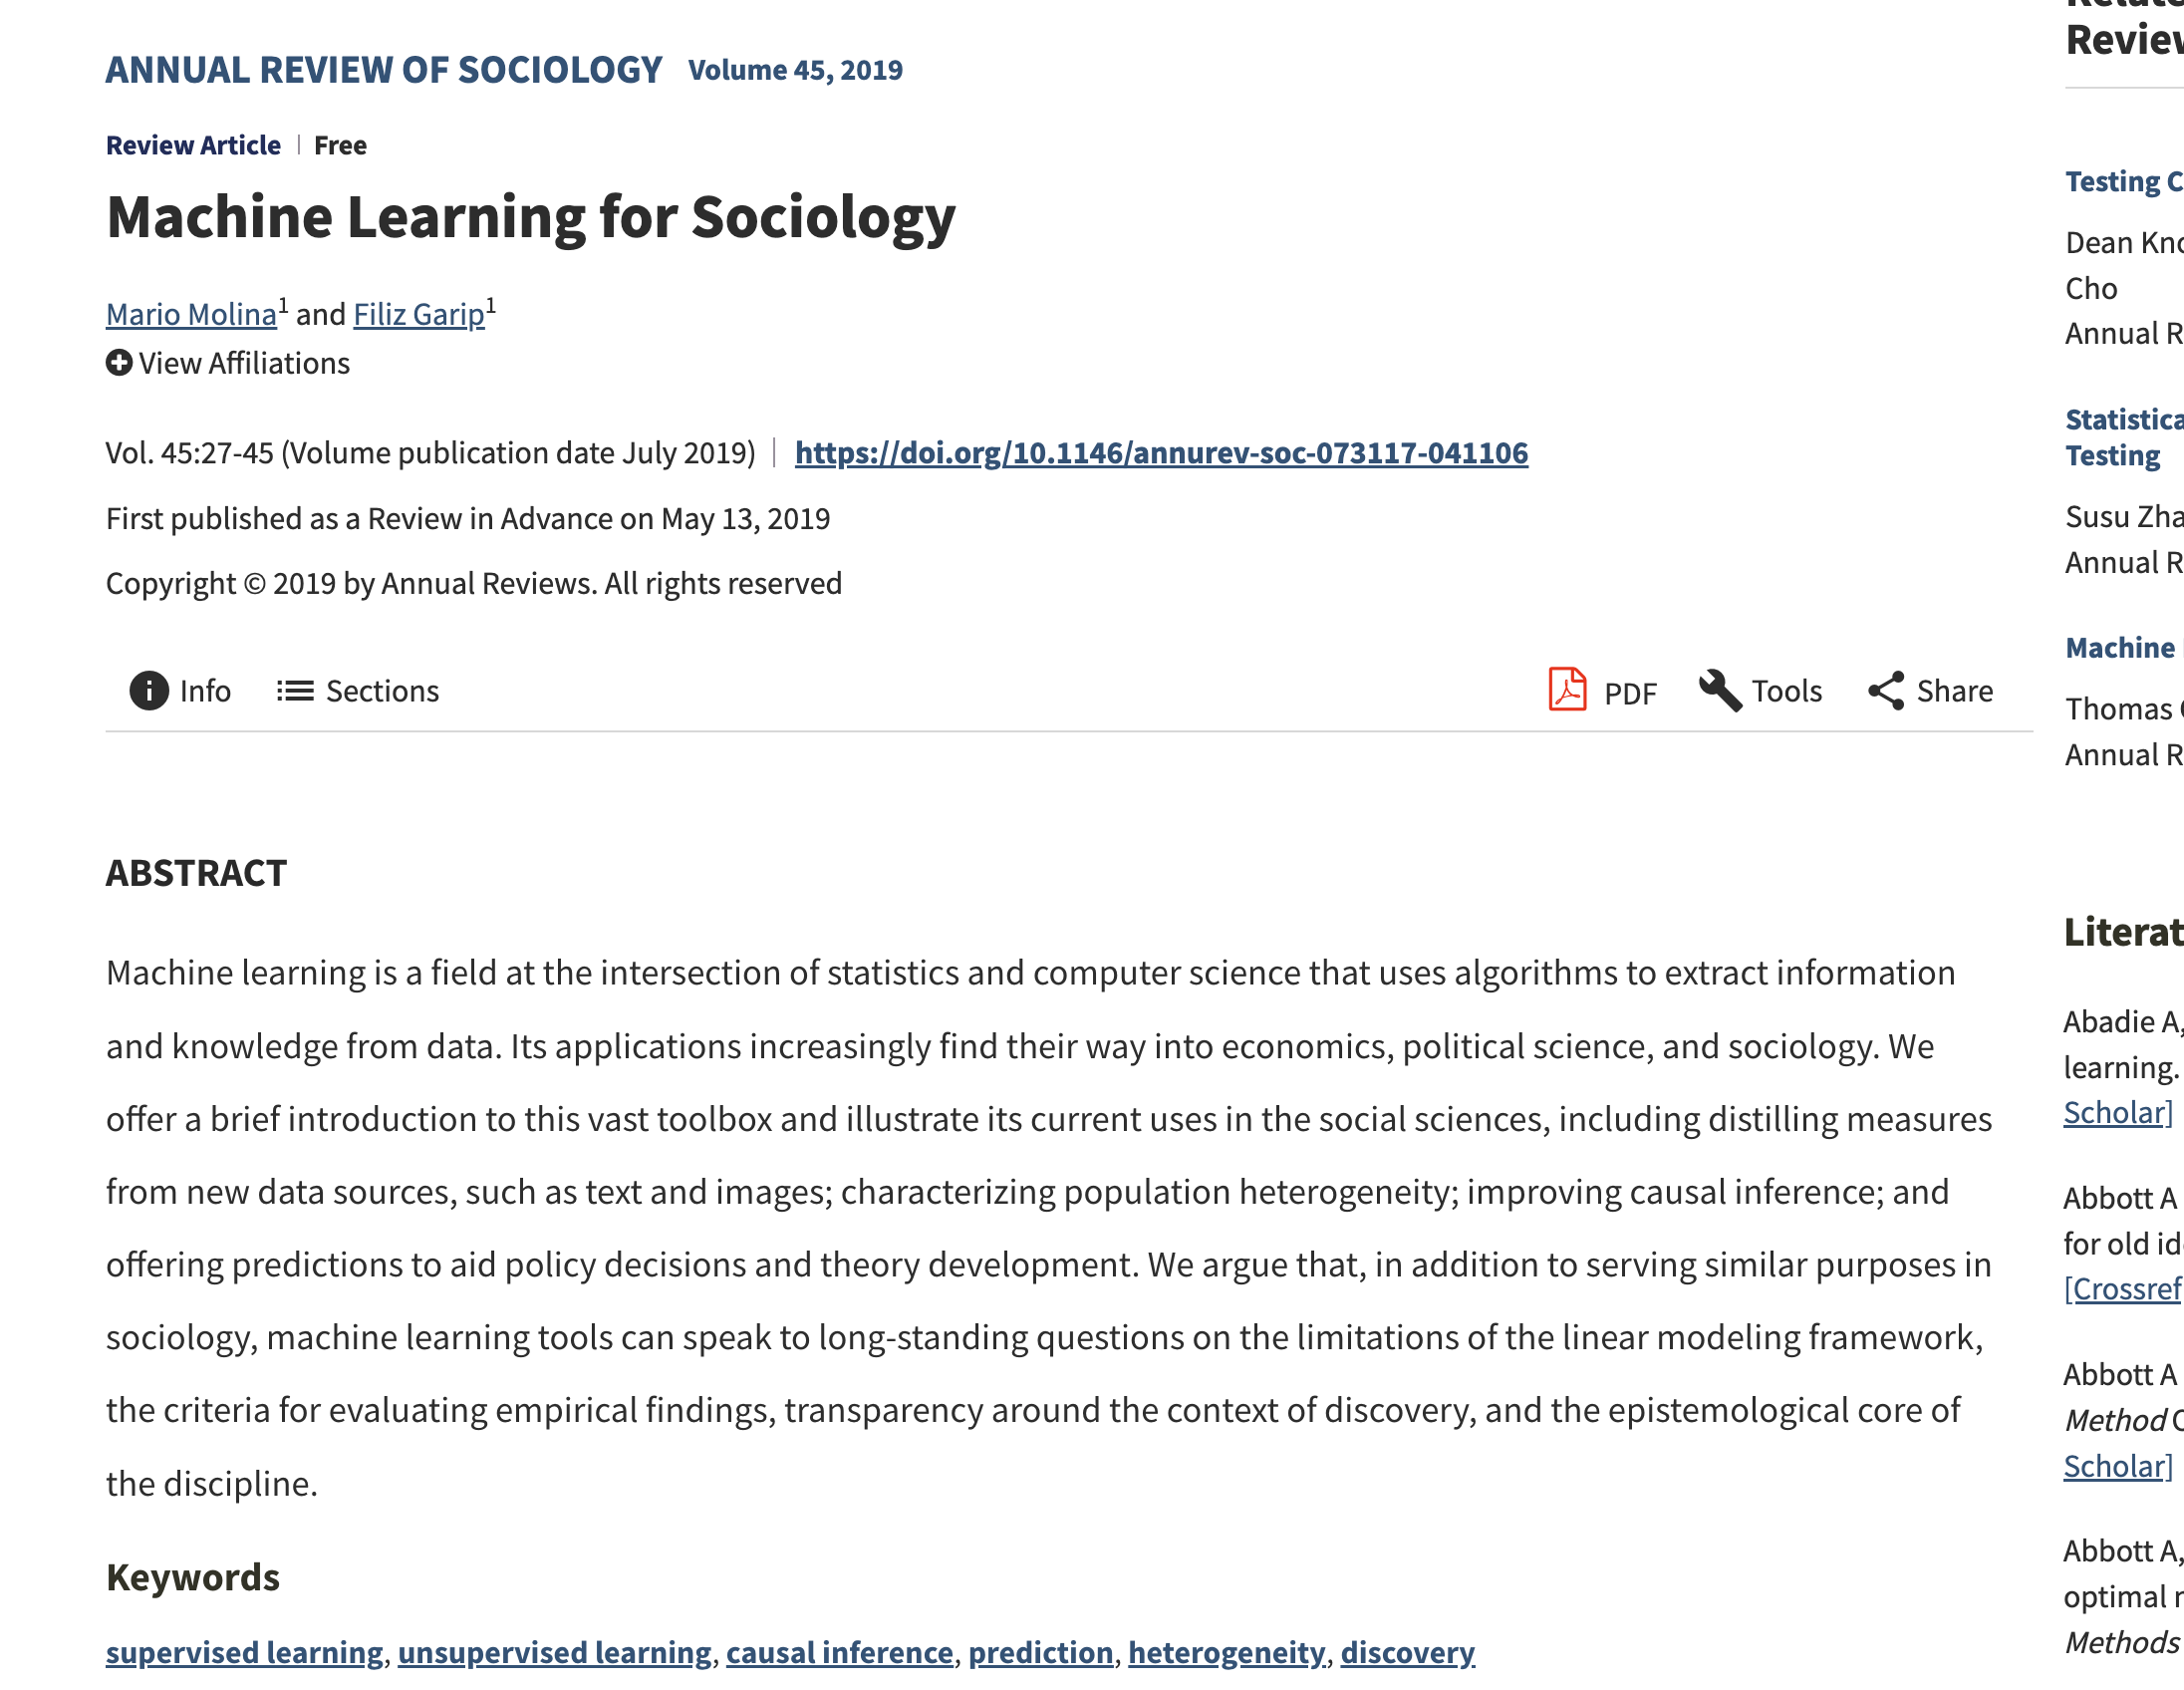
\includegraphics[keepaspectratio]{images/ml.png}}
\end{center}
\end{frame}

\begin{frame}{Some recent examples}
\phantomsection\label{some-recent-examples}
\begin{center}
\pandocbounded{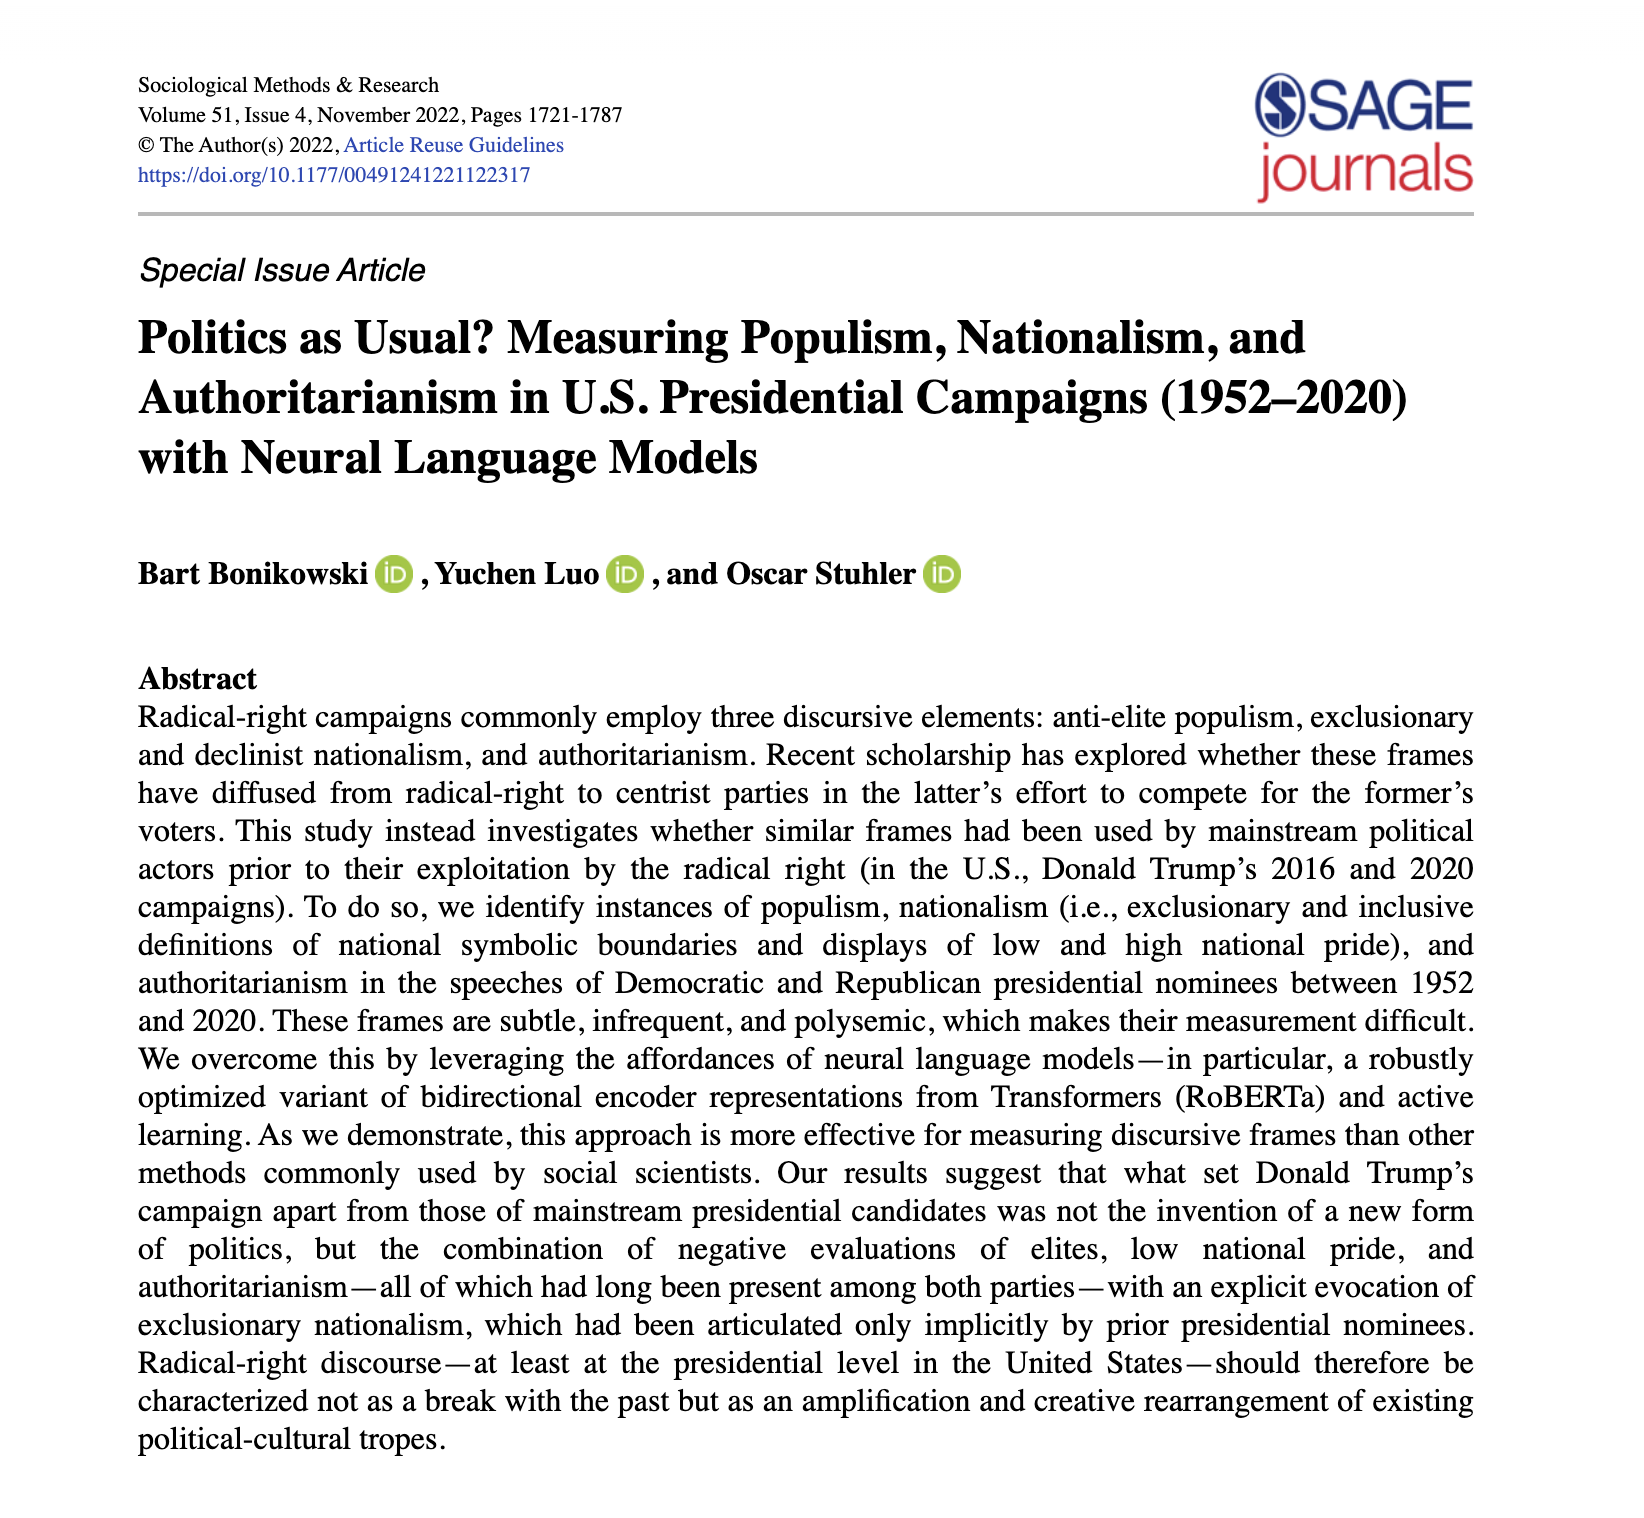
\includegraphics[keepaspectratio]{images/bonikowski.png}}
\end{center}
\end{frame}

\begin{frame}{Some recent examples}
\phantomsection\label{some-recent-examples-1}
\begin{center}
\pandocbounded{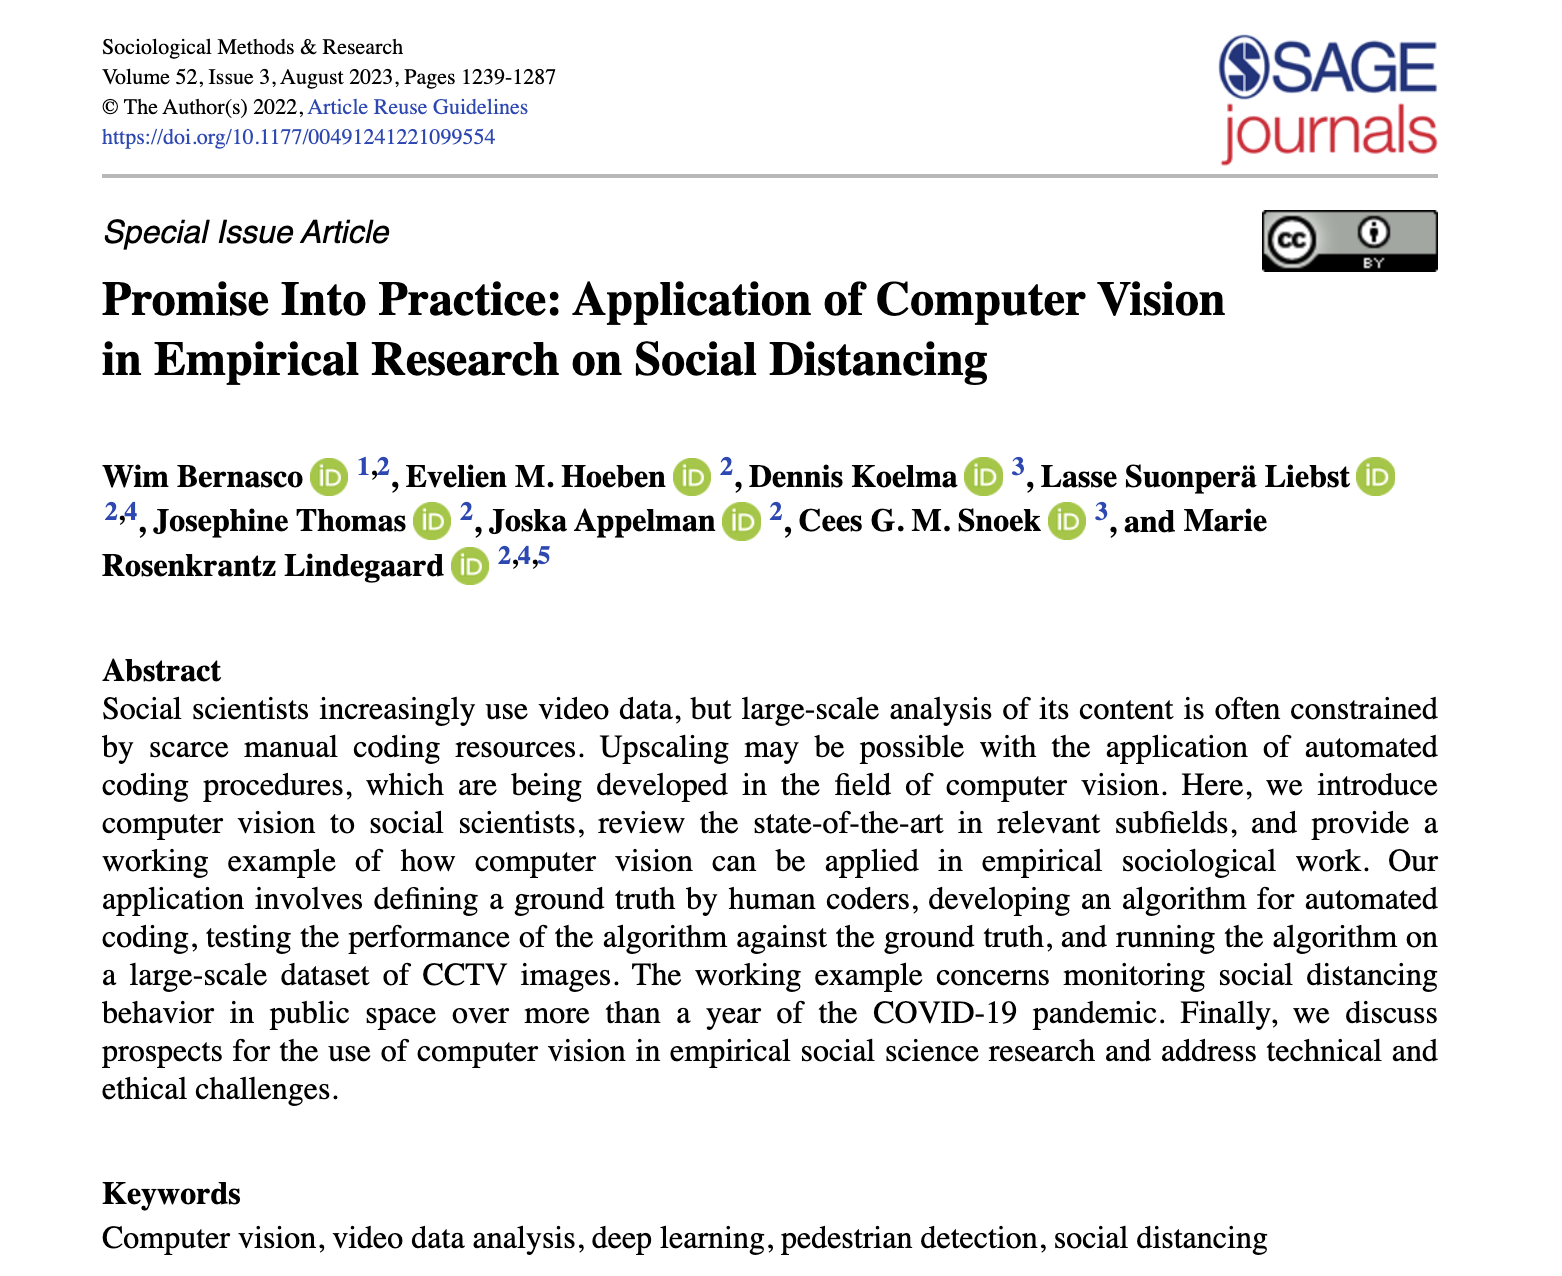
\includegraphics[keepaspectratio]{images/bernasco.png}}
\end{center}
\end{frame}

\begin{frame}{Some recent examples}
\phantomsection\label{some-recent-examples-2}
\begin{center}
\pandocbounded{
\includegraphics[keepaspectratio]{images/do.png}}
\end{center}
\end{frame}

\begin{frame}{Algorithmic bias}
\phantomsection\label{algorithmic-bias}
\end{frame}

\begin{frame}{Some recent examples}
\phantomsection\label{some-recent-examples-3}
\begin{center}
\pandocbounded{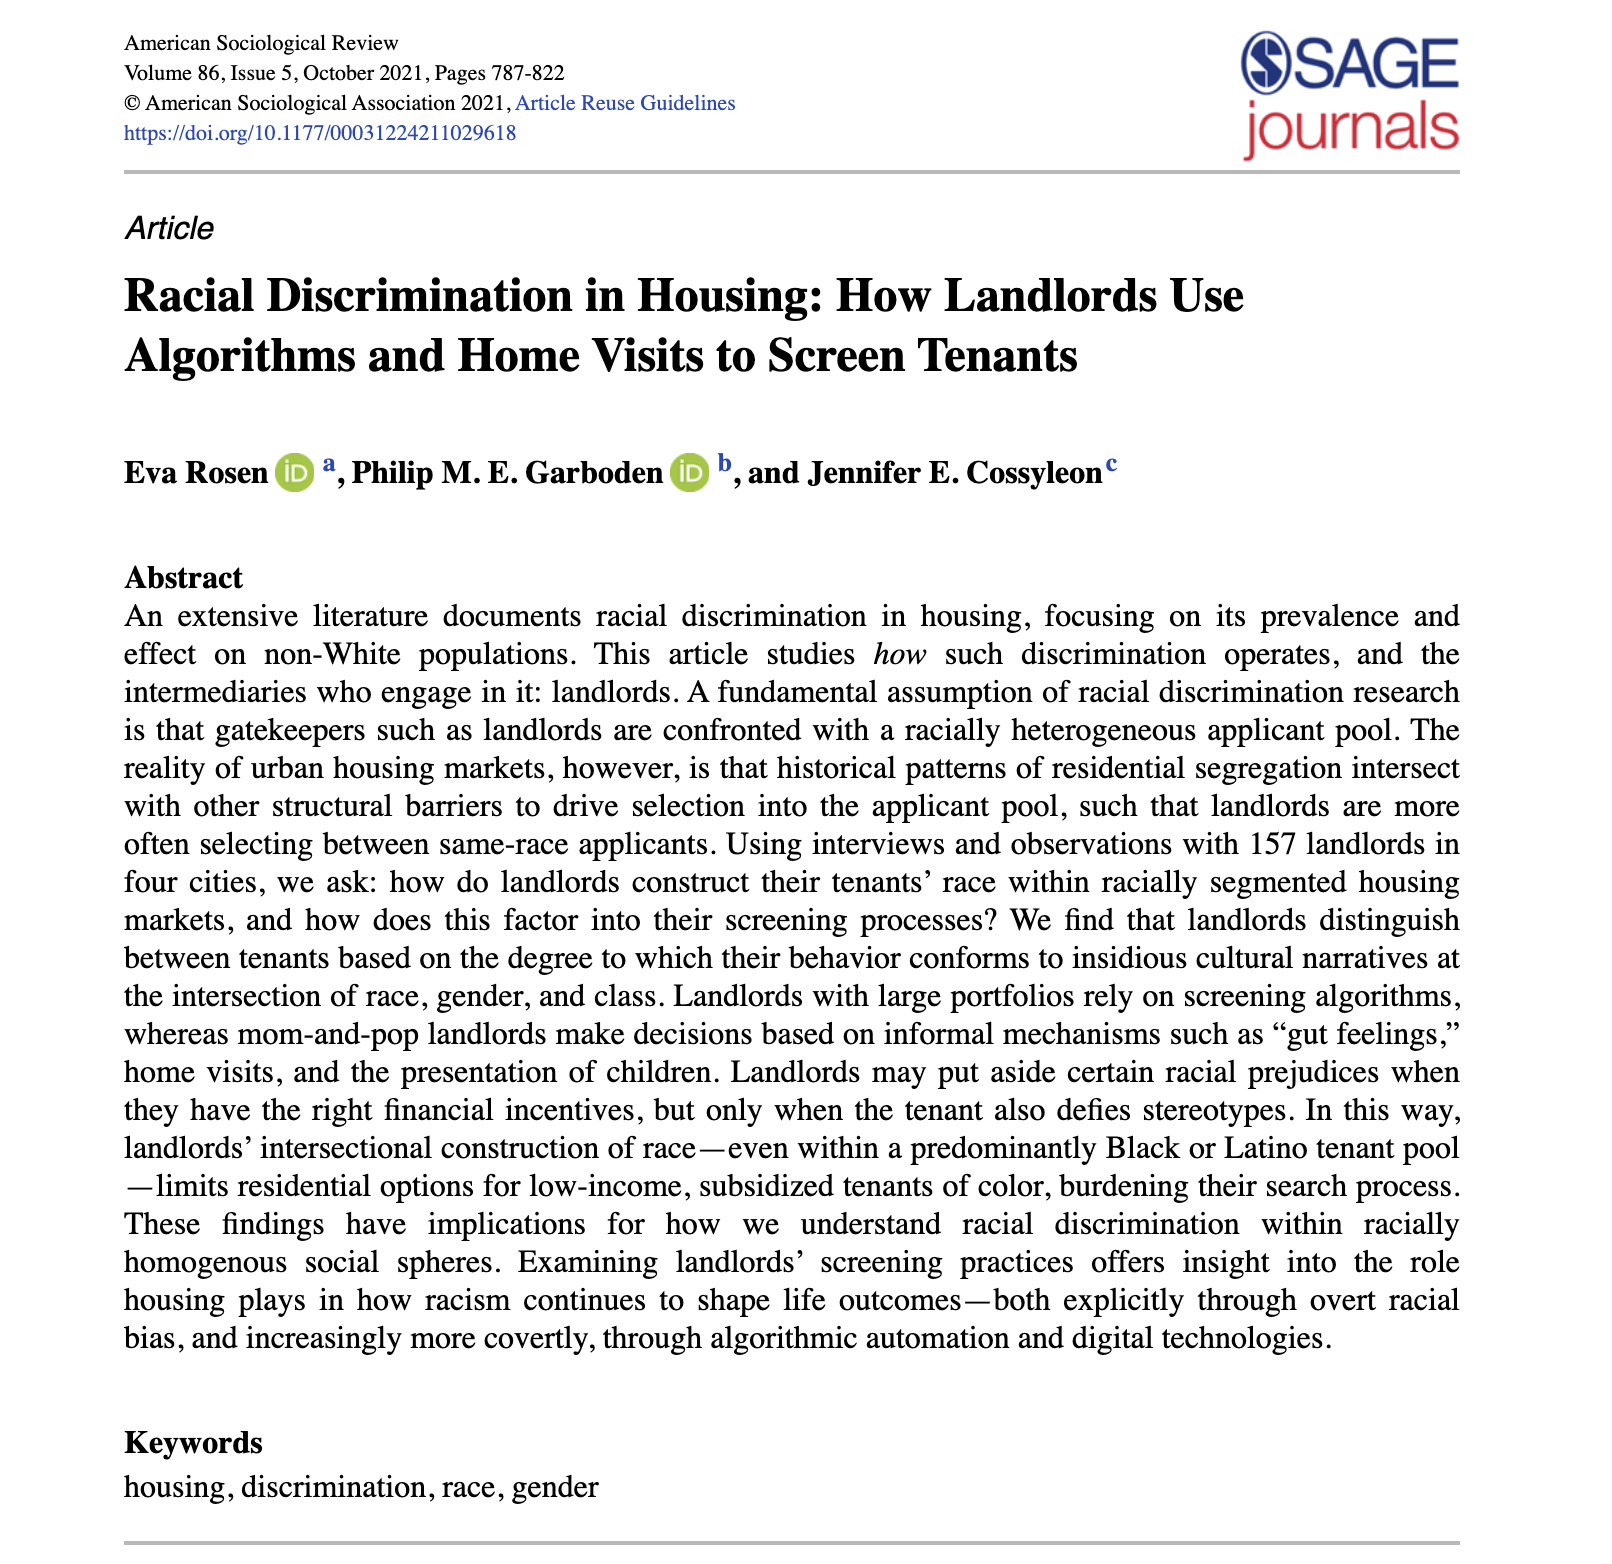
\includegraphics[keepaspectratio]{images/rosen.pdf}}
\end{center}
\end{frame}

\begin{frame}{Some recent examples}
\phantomsection\label{some-recent-examples-4}
\begin{center}
\pandocbounded{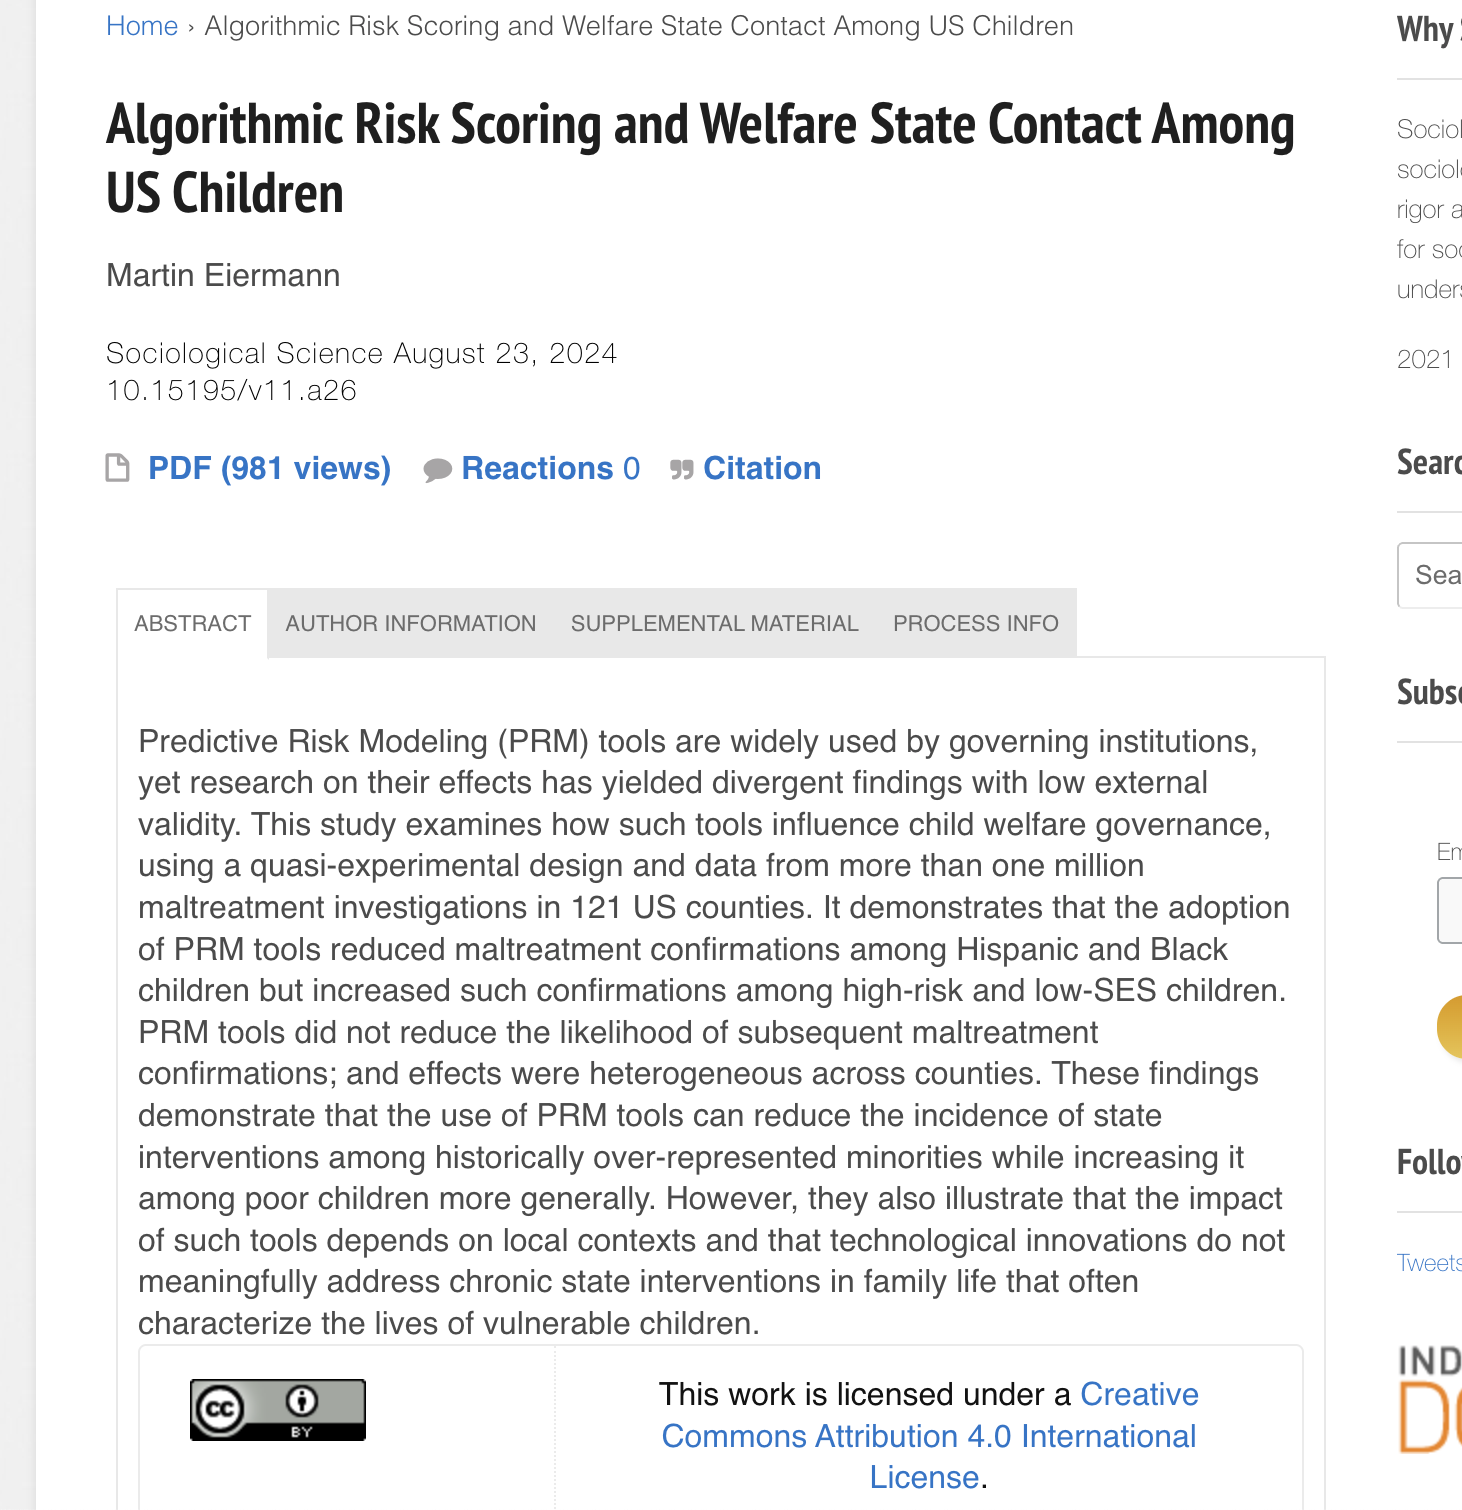
\includegraphics[keepaspectratio]{images/eiermann.pdf}}
\end{center}
\end{frame}

\begin{frame}{Some recent examples}
\phantomsection\label{some-recent-examples-5}
\begin{center}
\pandocbounded{
\includegraphics[keepaspectratio]{images/noble.pdf}}
\end{center}
\end{frame}

\begin{frame}{Simulation}
\phantomsection\label{simulation}
\end{frame}

\begin{frame}{Some early examples}
\phantomsection\label{some-early-examples-3}
\end{frame}

\begin{frame}{Some early examples}
\phantomsection\label{some-early-examples-4}
\begin{center}
\pandocbounded{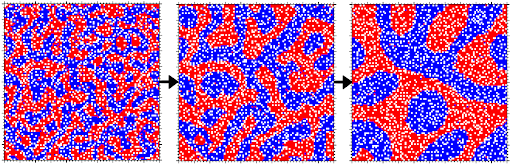
\includegraphics[keepaspectratio]{images/schelling.pdf}}
\end{center}
\end{frame}

\begin{frame}{Some early examples}
\phantomsection\label{some-early-examples-5}
\begin{center}
\pandocbounded{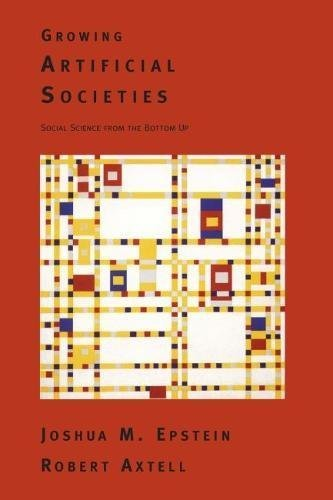
\includegraphics[keepaspectratio]{images/epstein.pdf}}
\end{center}
\end{frame}

\begin{frame}{Some more recent examples}
\phantomsection\label{some-more-recent-examples}
\begin{center}
\pandocbounded{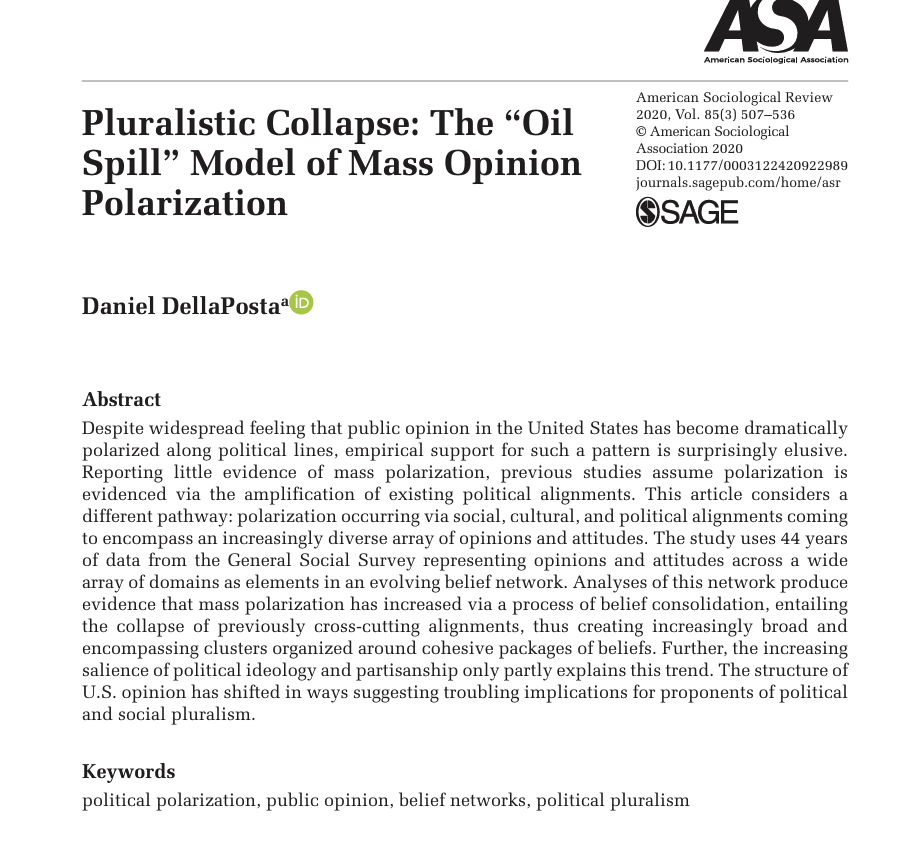
\includegraphics[keepaspectratio]{images/dellaposta.pdf}}
\end{center}
\end{frame}

\begin{frame}{So how do LLMs bring any of this together}
\phantomsection\label{so-how-do-llms-bring-any-of-this-together}
\begin{itemize}
\tightlist
\item
  LLMs both tool and object of inquiry (similar to ML)
\item
  LLMs can do (all? most?) of the above tasks
\end{itemize}
\end{frame}

\begin{frame}{What am I talking about?}
\phantomsection\label{what-am-i-talking-about}
\end{frame}

\begin{frame}{LLMs come from text as data}
\phantomsection\label{llms-come-from-text-as-data}
\begin{itemize}[<+->]
\tightlist
\item
  trained on massive corpora of text
\item
  learn patterns in text
\item
  generate text
\item
  can follow codebooks
\end{itemize}
\end{frame}

\begin{frame}{LLMs are also machine learning}
\phantomsection\label{llms-are-also-machine-learning}
\begin{itemize}[<+->]
\tightlist
\item
  trained using machine learning techniques
\item
  can be fine-tuned for specific tasks
\item
  can be used as components in larger ML systems
\end{itemize}
\end{frame}

\begin{frame}{LLMs can also be used in simulations}
\phantomsection\label{llms-can-also-be-used-in-simulations}
\begin{itemize}[<+->]
\tightlist
\item
  agents can be powered by LLMs
\item
  can simulate human-like behavior
\item
  can generate realistic scenarios
\end{itemize}
\end{frame}

\begin{frame}{LLMs can be objects of study}
\phantomsection\label{llms-can-be-objects-of-study}
\begin{itemize}[<+->]
\tightlist
\item
  how do they reflect biases in training data?
\item
  how do they impact society?
\item
  what are the ethical implications?
\end{itemize}
\end{frame}

\begin{frame}{This creates massive opportunities}
\phantomsection\label{this-creates-massive-opportunities}
\begin{itemize}[<+->]
\tightlist
\item
  We can annotate text at scale
\item
  We can build complex models of social phenomena
\item
  We can simulate complex social systems
\item
  We can study the impact of AI on society
\end{itemize}
\end{frame}

\begin{frame}{But also massive challenges}
\phantomsection\label{but-also-massive-challenges}
\begin{itemize}[<+->]
\tightlist
\item
  Ethical considerations
\item
  Bias and fairness
\item
  Interpretability
\item
  Reproducibility
\end{itemize}
\end{frame}




\end{document}
